\documentclass[conference,10pt]{IEEEtran}
\usepackage{amsmath,amssymb}
\usepackage{graphicx}
\usepackage{booktabs}
\usepackage{multirow}
\usepackage{xcolor}
\usepackage[hidelinks]{hyperref}
\usepackage[font=footnotesize,skip=3pt]{caption}
\newcommand{\cqlppo}{CQL$\to$PPO}
\newcommand{\bcppo}{BC$\to$PPO}
\setlength{\textfloatsep}{8pt plus 2pt minus 2pt}
\setlength{\floatsep}{6pt plus 2pt minus 2pt}
\setlength{\dbltextfloatsep}{8pt plus 2pt minus 2pt}

\begin{document}
\title{Learned Per-Frame QP Rate Control with Lookahead:\\ Results for x265 and x264}
\author{\IEEEauthorblockN{[Team members]}
\IEEEauthorblockA{EE599 Course Project, University of Southern California --- November 4, 2026}}
\maketitle

\begin{abstract}
We train reinforcement-learning (RL) agents that choose a quantiser (QP) for every frame of a 30-frame group of pictures (GOP) under a bit budget, with real x265 and x264 encodes, and measure how much each frame of lookahead is worth. An offline hindsight search saves about 10\% of bits at equal PSNR at every budget from QP 26 to QP 42. The best single-pass controllers, budget-constrained (Lagrangian / PID) RL, recover 40--50\% of that saving with 1--6\% of GOPs over budget, ahead of every other learner. Almost all the value of lookahead comes from the first 2--3 frames, and lookahead matters more as the budget gets tighter. RL's distinct contribution over imitation is budget reliability and allocation across GOPs. A peer review found that the budget features leak the GOP's total cost, so the causal ($k{=}0$) results are likely optimistic; we list this and the other caveats in Section~\ref{sec:threats}.
\end{abstract}

\section{Problem and setup}
\textbf{Episode.} One GOP of 30 frames (I + 29 P, no B-frames, AQ and CU/MB-tree off), $320{\times}180$, preset \emph{fast}, x265 4.1 and x264 0.165. At frame $t$ the agent sees the frames $t..t{+}k$ (first-pass bits, spatial/temporal complexity, scene flags) and the budget state, and picks a QP offset in $\{-3..3\}$ on top of a fixed pattern (STATIC: I $-6$, P1--9 $-3$, P10--29 $+3$) around base QP $b$. Each frame is encoded once, for real.
\textbf{Budget and score.} The budget is the bits the encoder's own constant-QP mode spends on the GOP at QP $b$. Score = \% bits saved at equal PSNR against the encoder's constant-QP curve (QP 18--50) $-\,2\times$\% over budget; we always report the share of GOPs more than 1\% over.
\textbf{Search.} A hindsight hill-climb (300 real encodes $\times$ 2 seeds per GOP and budget) sees the whole GOP; it is the target and the training data for offline RL.
\textbf{Data (v0).} 187 clips: YouTube UGC 360P, Xiph CIF/HD, Blender films, plus GOPs spliced from 2--3 clips with known cuts; 2{,}061 GOPs split by source (1{,}196 train / 386 val / 479 test). The first study used two budgets (QP 30, 38); the extension re-trains the core learners on five (QP 26, 30, 34, 38, 42), a median $7.8\times$ range of bits (42--349 kbit per GOP). All numbers are on test, averaged over 3 seeds; paired differences use a 95\% bootstrap over cases.
\textbf{Learners.} Imitation (BC on the search's best plans), offline RL (CQL, IQL), offline$\to$online (\bcppo, \cqlppo), online from scratch (PPO, A2C, DQN; 60k real-encode steps), constrained RL (Lagrangian and PID-Lagrangian PPO, the budget as a constraint), MPC with a learned bit/PSNR model, model-based PPO pre-training, and a seed ensemble.

\section{Results}
\subsection{Search gain and the encoders' own rate control}\label{sec:search}
The search scores 10.53 (x265) and 9.95 (x264) and stays at 9.2--11.0 at every one of the five budgets (Fig.~\ref{fig:budget}). It is still improving at 300 encodes (x265 mean best score $-6.8$, 3.5, 7.6, 10.0 after 10, 50, 100, 300), so it is a lower bound on the attainable gain, not a true ceiling. The encoders' own rate control (ABR, two-pass, ABR+VBV) scores below constant QP (Table~\ref{tab:methods}) and degrades as the budget tightens: x265 two-pass is over budget on 11\% of GOPs at QP 26 and 84\% at QP 42 (score $-14.0\to-34.8$); x264 two-pass is steadier ($-3.0$ to $-3.9$, 4--6\% over) except at QP 42 ($-8.1$, 12\%). This comparison is not fair to the encoders: constant QP at $b$ meets the budget by construction (an oracle), the encoders' defaults target subjective quality, and 30 frames give single-pass ABR little time to converge.

\begin{table}[t]
\centering\scriptsize
\caption{All learners (2-budget runs, QP 30/38; test, 958 cases). Score / share of cases $>$1\% over budget.}
\label{tab:methods}
\setlength{\tabcolsep}{2.2pt}
\begin{tabular}{@{}lcccc@{}}
\toprule
& \multicolumn{2}{c}{x265} & \multicolumn{2}{c}{x264}\\
\cmidrule(lr){2-3}\cmidrule(l){4-5}
Method & $k{=}0$ & $k{=}5$ & $k{=}0$ & $k{=}5$\\
\midrule
Constant QP (oracle base) & \multicolumn{2}{c}{0.00 / 0\%} & \multicolumn{2}{c}{0.00 / 0\%}\\
STATIC pattern & \multicolumn{2}{c}{$-$13.70 / 50\%} & \multicolumn{2}{c}{$-$15.95 / 56\%}\\
Own 2-pass & \multicolumn{2}{c}{$-$18.75 / 41\%} & \multicolumn{2}{c}{$-$3.44 / 5\%}\\
Own ABR+VBV & \multicolumn{2}{c}{$-$37.29 / 87\%} & \multicolumn{2}{c}{$-$37.80 / 79\%}\\
Hand lookahead rule & $-$6.00 / 27\% & $-$2.51 / 19\% & $-$5.39 / 25\% & $-$1.95 / 16\%\\
\midrule
BC (imitation) & 1.68 / 17\% & 3.77 / 9\% & 0.21 / 19\% & 2.65 / 21\%\\
CQL (offline) & $-$3.42 / 29\% & $-$1.77 / 26\% & $-$4.07 / 29\% & $-$1.23 / 25\%\\
IQL (offline) & 2.04 / 10\% & $-$0.63 / 23\% & $-$2.48 / 25\% & 0.35 / 18\%\\
\bcppo & 2.80 / 10\% & 3.17 / 14\% & 2.46 / 8\% & 3.60 / 10\%\\
\cqlppo & 0.74 / 22\% & 3.48 / 15\% & $-$1.17 / 25\% & 0.43 / 24\%\\
PPO (scratch) & 0.41 / 10\% & 0.32 / 14\% & $-$0.74 / 15\% & 0.15 / 14\%\\
A2C (scratch) & 0.53 / 3\% & $-$0.47 / 8\% & 1.04 / 1\% & $-$0.04 / 7\%\\
DQN (scratch) & 0.27 / 8\% & $-$1.41 / 11\% & 0.53 / 3\% & $-$0.23 / 6\%\\
\textbf{Lagrangian} & \textbf{4.36} / 1\% & \textbf{4.95} / 2\% & \textbf{3.90} / 2\% & 4.07 / 6\%\\
\textbf{PID-Lagrangian} & \textbf{4.46} / 4\% & 4.48 / 4\% & 3.83 / 4\% & \textbf{4.53} / 6\%\\
MPC (CEM) & $-$1.78 / 6\% & $-$0.43 / 7\% & $-$3.58 / 10\% & $-$2.46 / 10\%\\
Model-based + 40k real & 0.69 / 12\% & 0.96 / 7\% & 0.09 / 12\% & 1.00 / 7\%\\
Ensemble of 3 \cqlppo{} & -- & 4.52 / 11\% & -- & 3.44 / 14\%\\
\midrule
Hindsight search & \multicolumn{2}{c}{10.53 / 1\%} & \multicolumn{2}{c}{9.95 / 1\%}\\
\bottomrule
\end{tabular}
\end{table}

\begin{figure*}[t]
\centering
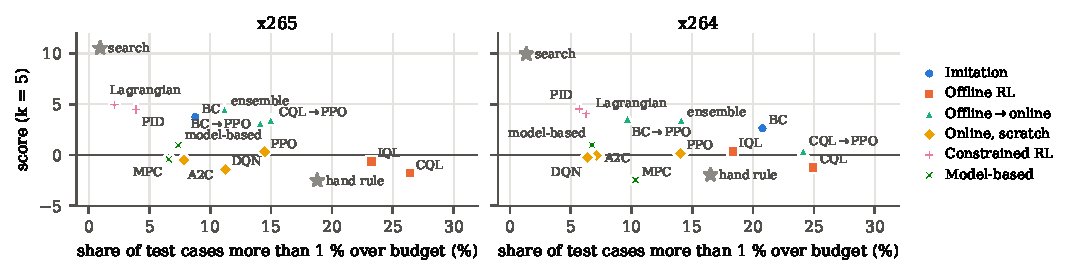
\includegraphics[width=0.92\textwidth]{fig_reliability.pdf}
\caption{Score against budget reliability for every learner at $k{=}5$ (2-budget runs, test). Top left is best. Constrained RL is the only family that is both high-scoring and almost always within budget; the encoders' own rate control lies off scale (score $-3$ to $-37$).}
\label{fig:rel}
\end{figure*}

\subsection{Which learning approach?}
Table~\ref{tab:methods} and Fig.~\ref{fig:rel} compare all learners. Four findings hold on both encoders.
(i) \emph{Online RL from scratch fails at this sample budget}: PPO, A2C and DQN stay within $\pm1.4$ of constant QP. They get 60k real encodes, while the offline learners use about 1.4M search encodes, so this is partly a compute result.
(ii) \emph{Imitation gives most of the saving}: BC saves 4.6--5.0\% at $k{=}5$; PPO fine-tuning adds about 0.5 points of saving but also overshoot.
(iii) \emph{Pure offline RL is worse than imitation}: CQL and IQL stay close to the logged plans, which are dominated by proposals near STATIC, and overshoot on 10--29\% of cases.
(iv) \emph{Constrained RL is the best single-pass controller}: Lagrangian beats BC by +2.68 [+2.21, +3.15] (x265) and +3.68 [+3.05, +4.35] (x264) at $k{=}0$, while also saving more bits and cutting over-budget cases by 16--17 points. MPC (CEM exploits its model's errors) and model-based pre-training (the model's $\approx$15\% bit error is larger than the effect of a good allocation, so it learns to spend less, not where to spend) are negative results.
A 3-seed ensemble of \cqlppo{} adds +1.04 [+0.73, +1.38] on x265. Removing first-pass features costs the most ($3.48\to-0.97$); scene and feedback features are roughly neutral.

\subsection{How much does each frame of lookahead buy?}
Fig.~\ref{fig:lookahead} shows \cqlppo{} against $k$. The first 2--3 frames carry nearly all of the benefit (x265, 2 budgets: +1.56 from $k{=}0\to1$ and +1.51 from $1\to2$). Beyond that the curve is flat within seed noise ($\pm1.5$), and the full GOP ($k{=}29$) is not better than $k{=}3$; on x264 with five budgets it drops to $-0.8$. The learned policy beats the hand-made lookahead rule given the same window by 3.7--9.2 points at every budget (Table~\ref{tab:budget}), so the value is in learning to use the lookahead, not in the window alone. Lookahead pays off at scene cuts: from $k{=}0$ to 5, \cqlppo{} gains +0.2 / +0.6 points of saving (x265 / x264) on stable GOPs but +3.2 / +3.8 on natural cuts and +4.9 / +5.5 on spliced cuts. Scene-aware windows cost less: a single policy trained with random window masking, with the window cut at the next scene change, scores 4.56 at $k{\le}5$ (x265), and a cut-triggered window keeps 3.32 while seeing on average 0.2 future frames instead of 4.5.

\begin{figure}[t]
\centering
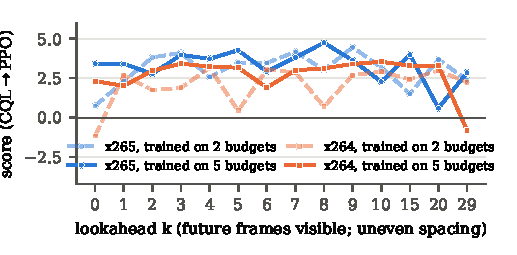
\includegraphics[width=\columnwidth]{fig_lookahead.pdf}
\caption{Lookahead curve of \cqlppo{} (test, QP 30 and 38 cases). Dashed: trained on 2 budgets; solid: trained on 5. The search scores $\approx$10 (off scale).}
\label{fig:lookahead}
\end{figure}

\subsection{Does it hold across budgets? (5-budget extension)}
Fig.~\ref{fig:budget} and Table~\ref{tab:budget} report the retrained core learners at each budget QP. The search gain is flat across budgets, but every learner loses ground as the budget tightens, so the gap to the search grows from +5.4 (QP 26) to +7.0 (QP 42) on x265 at $k{=}5$. Constrained RL is best at every budget, and its advantage over imitation grows as bits get scarcer (Lagrangian $-$ BC at $k{=}0$: x265 +2.3 $\to$ +5.4, x264 +2.6 $\to$ +5.9). Lookahead matters more at tight budgets: \cqlppo{} $k{=}5-k{=}0$ is +0.6 at QP 26 and +2.4 at QP 42 on x265, and is not significant at QP 26--30 on x264. Training on five budgets helps the penalty-based learner but not the constrained ones (Table~\ref{tab:train}): on the same QP 30/38 cases, \cqlppo{} at $k{=}0$ rises from 0.74 to 3.42 (x265) and from $-1.17$ to 2.31 (x264), mostly through fewer overshoots (22$\to$9\% and 25$\to$13\%), while Lagrangian and PID change by less than 0.8.

\begin{figure}[t]
\centering
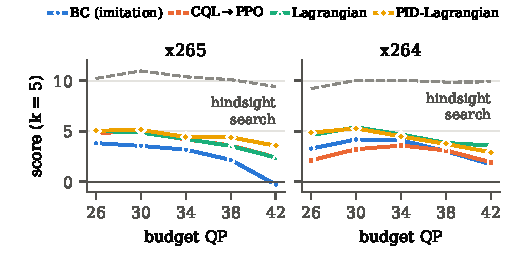
\includegraphics[width=\columnwidth]{fig_budget.pdf}
\caption{Score at each budget QP (higher QP = fewer bits), $k{=}5$, learners trained on 5 budgets (test, 479 GOPs per budget). The search gain is flat; learned controllers lose ground as bits get scarce.}
\label{fig:budget}
\end{figure}

\begin{table}[t]
\centering\scriptsize
\caption{Paired score differences per budget QP (5-budget runs, test). All 95\% bootstrap intervals exclude 0 except $^\dagger$.}
\label{tab:budget}
\setlength{\tabcolsep}{3pt}
\begin{tabular}{@{}llrrrrr@{}}
\toprule
& Difference (budget QP) & 26 & 30 & 34 & 38 & 42\\
\midrule
\multirow{4}{*}{x265} & Lagrangian $-$ BC, $k{=}0$ & +2.32 & +2.94 & +2.93 & +3.71 & +5.38\\
& \cqlppo{} $k{=}5-k{=}0$ & +0.64 & +0.62 & +0.82 & +1.07 & +2.41\\
& \cqlppo{} $-$ hand rule, $k{=}5$ & +5.04 & +6.14 & +6.24 & +7.41 & +9.15\\
& Search $-$ \cqlppo{} $k{=}5$ & +5.38 & +6.04 & +6.18 & +6.51 & +7.00\\
\midrule
\multirow{4}{*}{x264} & Lagrangian $-$ BC, $k{=}0$ & +2.63 & +4.22 & +2.92 & +4.61 & +5.87\\
& \cqlppo{} $k{=}5-k{=}0$ & $-0.36^\dagger$ & $+0.19^\dagger$ & +1.01 & +1.51 & +2.47\\
& \cqlppo{} $-$ hand rule, $k{=}5$ & +3.66 & +3.97 & +5.34 & +6.22 & +7.11\\
& Search $-$ \cqlppo{} $k{=}5$ & +7.09 & +6.83 & +6.45 & +6.76 & +7.95\\
\bottomrule
\end{tabular}
\end{table}

\begin{table}[t]
\centering\scriptsize
\caption{Training on 2 vs 5 budgets, evaluated on the same QP 30/38 test cases. Score (share $>$1\% over).}
\label{tab:train}
\setlength{\tabcolsep}{3pt}
\begin{tabular}{@{}lcc@{}}
\toprule
Method & x265: 2 $\to$ 5 budgets & x264: 2 $\to$ 5 budgets\\
\midrule
\cqlppo, $k{=}0$ & 0.74 (22\%) $\to$ \textbf{3.42} (9\%) & $-$1.17 (25\%) $\to$ \textbf{2.31} (13\%)\\
\cqlppo, $k{=}5$ & 3.48 (15\%) $\to$ \textbf{4.26} (10\%) & 0.43 (24\%) $\to$ \textbf{3.15} (14\%)\\
BC, $k{=}5$ & 3.77 (9\%) $\to$ 2.85 (16\%) & 2.65 (21\%) $\to$ 3.60 (8\%)\\
Lagrangian, $k{=}5$ & 4.95 (2\%) $\to$ 4.19 (2\%) & 4.07 (6\%) $\to$ 4.61 (3\%)\\
PID, $k{=}5$ & 4.48 (4\%) $\to$ 4.76 (2\%) & 4.53 (6\%) $\to$ 4.51 (6\%)\\
\bottomrule
\end{tabular}
\end{table}

\subsection{Budgets shared across GOPs}
\begin{table}[t]
\centering\scriptsize
\caption{Multi-GOP streams (8 GOPs, one budget; test, 912 cases). Score / share $>$1\% over. $L$: GOPs of lookahead.}
\label{tab:multigop}
\setlength{\tabcolsep}{4pt}
\begin{tabular}{@{}lcc@{}}
\toprule
Method & x265 & x264\\
\midrule
Hand rule, $L{=}0$ / $L{=}2$ & $-$20.68 / $-$10.37 & $-$44.86 / $-$14.08\\
BC (imitation), $L{=}0$ / $L{=}2$ & $-$16.99 / $-$19.56 & $-$16.06 / $-$19.63\\
Best constant QP (hindsight) & 0 / 0\% & 0 / 0\%\\
PPO, $L{=}2$ & 3.04 / 1\% & 1.87 / 1\%\\
\textbf{\bcppo, $L{=}2$} & \textbf{3.23} / 1\% & \textbf{1.86} / 1\%\\
Hindsight per-GOP plan & 12.54 / 0\% & 12.45 / 0\%\\
\bottomrule
\end{tabular}
\end{table}
In a second setting (Table~\ref{tab:multigop}), 8 consecutive GOPs share one budget whose matching QP is unknown. Here imitation of the hindsight per-GOP plan fails ($-17$ to $-20$), and the hand rule loses $-20.7$ (x265) / $-44.9$ (x264) without lookahead. RL is the only causal controller above the best constant QP chosen in hindsight: \bcppo{} with 2 GOPs of lookahead scores +3.23 [+2.79, +3.64] (x265) and +1.86 [+1.34, +2.36] (x264) at 1\% over budget.

\section{Threats to validity}\label{sec:threats}
A code review found these issues; none is fixed above.
(1)~\emph{Budget leak.} The budget is the GOP's own constant-QP spend, and it enters the observation (budget / first-pass bits of frame 0, and every frame's cost is normalised by it), so even a $k{=}0$ policy knows the GOP's total cost. This probably inflates causal results and may be why the curve flattens after $k{\approx}3$.
(2)~\emph{Oracle base QP.} The base $b$ is exactly the QP that meets the budget, so ``constant QP'' is an oracle and the comparison with the encoders' own rate control favours us.
(3)~\emph{Scene flags look ahead} 2--4 frames (flash and fade detection), so $k{=}0$ is not strictly causal; the scene-feature ablation suggests the effect is small.
(4)~\emph{STATIC is a weak base} on both encoders ($-11.4$ / $-14.4$ on train vs.\ +1.7 / +2.5 for the best refit).
(5)~\emph{Statistics.} Intervals resample cases, not clips (one film supplies 131 of 479 test GOPs), so they are too narrow; 60 of the 90 test GOPs with cuts are spliced.
(6)~\emph{Search not converged} (Section~\ref{sec:search}) and $\lambda$ / PID target fixed, not tuned on validation.

\section{Conclusions and next steps}
\textbf{Relation to prior work (discussion only).} We did not reproduce the following methods, and their published results are not comparable to ours: they use a different codec (libvpx VP9), baseline (libvpx two-pass VBR), metric (BD-rate) and episode (whole videos). Mao et al.~\cite{mao2020neural} train a neural rate controller by imitating per-video search plans. They report that imitation alone often misses the bit-rate target, and they add auxiliary bit losses, hindsight relabelling of the target, inference-time feedback control and training on many target bit rates. Our observations are consistent with theirs: plain BC on search plans keeps much of the saving but misses the budget, and training on more budgets reduced overshoot. Our remedy for the budget is different, closed-loop constrained RL. MuZero rate control~\cite{mandhane2022muzero} plans with a learned encoder model and a self-competition reward. Our much simpler model-based variants (MPC, model-based pre-training) failed because the learned model's error exceeded the effect of a good allocation, which says nothing about MuZero itself. Both works give the controller the whole video's first-pass statistics; our question, the lookahead--quality trade-off under a fixed GOP budget, is complementary.

\textbf{(1)} A single-pass learned controller recovers 40--50\% of the search's bit saving (score share 39--47\%), and constrained RL is the best and most reliable choice at every budget on both encoders.
\textbf{(2)} Lookahead is worth 2--3 frames; longer windows do not help with this data and training budget, but lookahead matters more when bits are scarce.
\textbf{(3)} RL's distinct value over imitation is keeping the budget (per GOP) and allocating it across GOPs, where imitation fails outright.
\textbf{(4)} Training on a range of budgets fixes most of the penalty-based learner's overshoot; the constrained learners already handle the budget and do not need it.
\textbf{(5)} Online RL from scratch, MPC and model-based pre-training do not work at this sample budget and model accuracy.
\textbf{Next:} remove the budget leak, use an estimated base QP and online scene flags, then rerun the core learners on dataset v1 (1{,}042 GOPs, human-reviewed cuts, natural cuts in test) with a clip-level bootstrap. If the $k{=}0$ results fall after the fix, the value of lookahead in finding (2) is larger than reported here.
\par
{\footnotesize
\begin{thebibliography}{1}
\bibitem{mao2020neural} H. Mao \emph{et al.}, ``Neural rate control for video encoding using imitation learning,'' arXiv:2012.05339, 2020.
\bibitem{mandhane2022muzero} A. Mandhane \emph{et al.}, ``MuZero with self-competition for rate control in VP9 video compression,'' arXiv:2202.06626, 2022.
\end{thebibliography}}
\end{document}
